\chapter{Introducción}

\section{Motivación}

\noindent 

La navegación autónoma de vehículos ha emergido como uno de los desafíos más apasionantes y complejos en el campo de la robótica. 
Con la creciente demanda en este ámbito, se han desarrollado múltiples empresas con proyectos que intentan ofrecer soluciones a un 
problema tan interesante como es la posibilidad de que un robot móvil se desplace autónomamente trazando un recorrido o ruta establecida. 
Según la \cite{IFR23} existe un 5\% de crecimiento en el volumen anual de ventas de robots industriales y así como hace unos años este crecimiento 
sería principalmente de manipuladores cada vez más la robótica móvil busca su camino en la industria dando soluciones super versátiles y de muy fácil 
implementación para tareas que antes requerían espacios enormes, donde ahora un robot móvil de bajas dimensiones puede soportar cargas muy grandes 
y ser implementado en la producción sin necesidad de modificar el entorno lo más mínimo. 

Otro punto importante es la problemática en la navegación que incluye conseguir un método fiable de localización donde la solución consiste en estimar la posición final del
robot compensando los errores incrementales de odometría acumulados, minimizar los errores producidos por el sistema sensorial y la detección de 
obstáculos mediante una sensorización a distancia que nos permita evitarlos y de esta manera planificar un camino de manera segura.

A diferencia de los espacios interiores, donde el entorno está controlado y predefinido, la navegación en exteriores presenta una serie de 
desafíos únicos que requieren soluciones innovadoras y adaptativas. Entre estos desafíos se encuentran la variabilidad del entorno, los 
cambios en las condiciones climáticas, la presencia de obstáculos dinámicos, la diversidad de superficies en el terreno y la localización 
en un entorno con tantas fuentes de ruido e interferencias.


Por estas razones cada vez más equipos de investigación se centran en conseguir nuevas formas de mejorar y de estandarizar las soluciones 
que existen, desde robots de rescate, militares o vehículos para uso personal, y aunque existen multitud de formas de afrontar este 
problema, existe un amplio margen de mejora. Por nuestra parte, en el presente trabajo se ha tomado especial atención a la parte de localización,
adaptando metodologías de estimación como el filtro extendido de Kalman,\Cite{Rolan20}, dado que este presenta múltiples complicaciones a la hora de
 realizarlo en exteriores como ya se ha comentado, también se han implementado algoritmos que intentan mejorar los errores producidos por los sensores y
finalmente algoritmos de planificación de trayectorias que se adecuen bien con el modelo del robot (Ackermann).

\newpage

\section{Objetivos del estudio}
Para considerar como finalizada la realización de este trabajo se van a establecer unos objetivos a conseguir, estos son:
\begin{itemize}
  \item Sistema de sensorización, se dispondrá de un montaje en el chasis del robot de manera que asegure un buen uso de los dispositivos y 
se realizará una implementación de drivers para su uso con el SDK ROS2, se debe buscar una manera efectiva de montar, conexionar y conectar 
con el software. 
  \item Interfaz de usuario, se debe buscar una manera fiable, versátil e intuitiva para que un usuario pueda probar y controlar el robot de 
manera rápida y sencilla, también se buscará la posibilidad de que la interfaz sea fácilmente modificable para futuras actualizaciones.
  \item Localización, objetivo fundamental para la navegación, se abordará la fusión de datos sensoriales heterogéneos para obtener una 
localización precisa y fiable.
  \item Evitación de obstáculos, se buscará una navegación segura, es decir, se configurarán sensores y algoritmos de navegación para 
conseguir una evitación de obstáculos estáticos y dinámicos.
  \item Navegación punto a punto y en trayectorias establecidas, se desarrollara un sistema de algoritmos que consigan una navegación 
basada en waypoints, el robot deberá visitar estos puntos de manera consecutiva  y deberán estar basados en coordenadas GPS (latitud, 
longitud, altitud).
\end{itemize}
\newpage

\section{Estructura del trabajo}

Este proyecto ha sido dividido en 6 capítulos bien definidos:

Primero, una introducción donde se presenta el tema y se dejan claros los objetivos del proyecto y los antecedentes en relación al tema del 
trabajo.

Segundo, el estado del arte donde se desarrollan los temas que en el presente trabajo se exponen, sus antecedentes históricos y su base de 
funcionamiento práctico
Tercer, el desarrollo en si del trabajo donde se explican en detalle el hardware utilizado, los métodos y herramientas y la manera en la que 
se ha trabajado para completar el proyecto. Está parte ha sido escrita de manera cronológica en cuanto a los pasos que se han seguido junto 
con las soluciones que se han ido dando a los diversos problemas que han aparecido durante el recorrido de este proyecto.

Cuarto, las pruebas del proyecto que incluyen datos experimentales, gráficas y simulaciones donde se comparan tanto las ideas teóricas con 
los resultados reales como las simuladas con las reales, se hace un estudio exhaustivo de donde hubo más complicaciones a la hora de llevar 
el proyecto a la realidad y como se fueron solucionando cada uno de los problemas.

Quinto, conclusiones finales del proyecto donde se reflexiona sobre las soluciones obtenidas y en cuanto son de fiables en un entorno tan 
variable.

Sexto, futuras lineas del trabajo donde se podría continuar este proyecto y mejorarlo.

\chapter{Estado del arte}
\section{Navegación Autónoma de vehículos Ackermann}
\subsection{Antecedentes}
La robótica y la navegación autónoma han sido áreas de investigación fascinantes y de rápido avance en las últimas décadas. 
Desde los primeros experimentos pioneros hasta los desarrollos más recientes, estas tecnologías han abierto un amplio espectro de 
posibilidades en diversos campos, desde la exploración espacial como el rover perseverance~\Cite{nasa24} de la NASA hasta la logística 
industrial con los manipuladores móviles de Robotnik~\Cite{robotnik24}.

Uno de los puntos de partida fundamentales en la historia de la robótica autónoma fue el trabajo realizado por el neurofisiólogo británico 
William Grey Walter en la década de 1940~\cite{holland2003first}. Walter diseñó y construyó los "robots tortuga", pequeños dispositivos 
autónomos que demostraron comportamientos primitivos de evasión de obstáculos y búsqueda de energía, destacando la capacidad de los robots 
para adaptarse y responder al entorno sin control humano directo.

\begin{figure}[h]
    \centering
    \includegraphics[width=0.4\textwidth]{images/tortugas_william_grey.jpg}
    \caption{Interior de los robots "tortuga".}
    \label{fig:tortugas_grey}
\end{figure}


Otro hito importante en este campo fue el desarrollo de la furgoneta autónoma Mercedes-Benz de Ernst Dickmanns y su equipo en la década de 
1980~\Cite{ernst80}. Este vehículo, equipado con sensores y sistemas de control avanzados, fue capaz de navegar de forma autónoma por 
carreteras y seguir a otros vehículos con un alto grado de precisión, sentando las bases para los sistemas de conducción autónoma modernos. 
Este vehículo fue   incluso capaz de circular por una ''autobahn'' alemana a 90 km/h

\begin{figure}[h]
    \centering
    \includegraphics[width=0.5\textwidth]{images/furgoneta_ernst_dickens.jpeg}
    \caption{Furgoneta Autónoma creada por Ernst Dickmanns~\cite{ernst80}.}
    \label{fig:furgoneta_ernst}
\end{figure}

En el ámbito militar, la Agencia de Proyectos de Investigación Avanzada de Defensa (DARPA) de los Estados Unidos ha desempeñado un 
papel crucial en el impulso de la robótica y la navegación autónoma. Uno de los proyectos emblemáticos de DARPA fue el primer vehículo 
que funcionaba mediante un radar, un láser, y visión computarizada. En 1987, los laboratorios HRL demostraron que se podía construir un 
vehículo que podía diseñar su propia ruta una vez que se salía del mapa~\cite{DARPA20}. El vehículo pudo moverse más de 600 metros a través de terreno 
complejo como pendientes, grandes rocas y vegetación.

\subsection{Actualidad}

Pronto grandes empresas como Google, Audi o más adelante Tesla iniciaron una nueva revolución en el mundo de la conducción autónoma, 
introduciendo los conceptos de \textit{machine learning} o \textit{deep learning} en sus vehículos como una nueva forma de toma de 
decisiones, de esta manera los vehículos primero aprendían ellos solos a que hacer en cada situación en base a un entrenamiento previo, 
esto dio lugar a una gran ventaja ya que en este campo la programación clásica era inviable por la gran cantidad de casos que existen.

Audi comenzó esta travesía con su modelo RS7 autónomo~\cite{audirs715}, que recorrió a una velocidad de 240 km/h el circuito de Hockenheim en Alemania. 
Siendo este 5 segundos más rápido que un un vehículo tripulado por un conductor profesional. A este le siguió Google con una flota de 25 
vehículos autónomos que sin superar los 40 km/h recorrieron las calles de Mountain View, California.

Más adelante salieron empresas como Waymo~\cite{waymo24}, que empezaron a desarrollar el concepto de un taxi autónomo~\cite{}, Tesla con sus vehículos que 
incorporan el conocido \textbf{Autopilot}, este utiliza una combinación de cámaras, radares y sensores para ofrecer características 
avanzadas de asistencia al conductor, como el piloto automático adaptativo y la asistencia de cambio de carril.

\section{Nav2: Stack para navegación autónoma de robots móviles}
ROS es un SDK o framework para el desarrollo de software para robots, este fue desarrollado en 2007 en la universidad de Standford para 
dar soporte a un proyecto interno, desde el 2008 ha sido mantenido principalmente por Willow Garage, una incubadora de empresas y 
laboratorio de investigación robótica, aunque por su naturaleza de código abierto el crecimiento y el mantenimiento ha sido una labor 
común de sus usuarios~\cite{ros2}.

ROS2 funciona en base a Nodos, programados en C++ o Python, estos comprenden los llamados paquetes y el conjunto de paquetes es un stack, 
uno de los stacks más conocidos, usados y mejorados es el utilizado en este trabajo, Nav2 o Navigation2~\cite{nav2}~, que en ya su segunda 
versión es la opción más utilizada para la creación de algoritmos de navegación autónoma.
Este stack comprende todo lo necesario para crear un sistema robusto de navegación autónoma principalmente en interiores pero también para exteriores,
comprende soporte para todo tipo de robots (Ackermann, Diferencial, Humanoide, Omni-direccional), aquí nos referiremos a los planificadores locales
como ''controladores'' y a los planificadores globales como simplemente ''planificadores''. Nav2 cuenta con controladores muy rápidos y 
sencillos como el DWB (Dynamic Window Approach) que funciona exclusivamente para robots que pueden girar \textit{in situ}, el TEB 
(Time Elastic Band) o el famoso RPP (Regulated Pure Pursuit) que aunque sencillos ya nos permiten una configuración más avanzada y necesaria
para nuestro caso como es el ángulo de giro mínimo, hasta otros mucho más complejos como el MPPI (Model Predictive Path Integral), un algoritmo 
muy complejo que usa un método de predicción en el tiempo para navegación de vehículos a grandes velocidades. Por otro lado tenemos los 
planificadores donde tenemos varias versiones de 2 algoritmos también muy conocidos, el A* y el Theta*~\cite{sun2023path}.

En su primera versión este stack usaba una máquina de estados finita como lógica de actuación, una solución muy bien estudiada por su antigüedad
pero que su modificación para un problema concreto resultaba complicada, por ello en su nueva versión se utilizan los llamados 
\textit{behavior trees}~\cite{colledanchise2018behavior}, unas estructuras de lógica muy versátiles y sobre todo extremadamente customizables, 
gracias a ello el stack de navegación permite una configuración absoluta de todos sus componentes, desde la creación de planificadores locales, globales, 
plugins para añadir comportamientos, capas para los mapas de coste, suavizadores de trayectoria o incluso la creación o modificación de los 
propios arboles de comportamiento.
\begin{figure}[h]
    \centering
    \includegraphics[width=0.8\textwidth]{images/nav2_architecture.png}
    \caption{Arquitectura interna de Nav2.}
    \label{fig:nav2_arch}
\end{figure}
\newpage
\section{Localización}
La localización se conoce como uno de los principales y más complejos problemas de la robótica móvil, este se basa en un concepto 
muy sencillo, saber donde se encuentra el robot, una tarea que depende del entorno, de las condiciones y de los sensores disponibles 
puede suponer un gran problema, por ello durante los años se han creado multiples técnicas de localización para intentar mitigar este 
gran problema, aquí se exponen los principales métodos usados a día de hoy en robótica.

\subsection{SLAM: Simultaneous Localization And Mapping}
El SLAM, es un método utilizado en robótica y campos relacionados para que un agente móvil (como un robot) pueda construir un mapa de un 
entorno desconocido y al mismo tiempo determinar su propia posición respecto de ese mapa.

El proceso comienza con una estimación inicial de la posición del robot y el mapa del entorno. Esta estimación puede ser rudimentaria y 
se mejora a medida que el robot explora y recopila más datos, luego sucede una captura de datos donde el agente móvil o robot, utiliza sus 
sensores como cámaras, LIDAR o diferentes fuentes de odometría para capturar información sobre la disposición del entorno y su propia 
posición. A partir de los datos capturados se construye un modelo del entorno que puede ser 2D o 3D. A medida que el agente móvil se mueve 
y recopila más datos, el mapa y la estimación de la posición se actualizan continuamente para reflejar el conocimiento más reciente del 
entorno y la ubicación del agente. El algoritmo incluye técnicas avanzadas de fusión sensorial, estimación probabilística y optimización 
para lograr una localización y un mapeo precisos

Este método es uno de los más usados en navegación en interiores donde hay muchos objetos y referencias donde el algoritmo constantemente 
puede "encontrarse", el principal problema recae cuando se intenta usar en exteriores donde suele haber pocas referencias o están mucho más 
espaciadas, donde el ruido es mucho mayor y existen más fuentes y sobre todo donde la idea de mapear un entorno tan extenso se vuelve 
inviable para la mayoría de situaciones.

\subsection{AMCL: Adaptive Monte Carlo Localization}

AMCL es un método probabilístico para la localización de robots que utiliza un enfoque de Monte Carlo (también conocido como filtro de 
partículas). A diferencia de otros métodos, AMCL puede adaptarse dinámicamente a la incertidumbre y las fluctuaciones en el entorno. 

Primeramente se genera un conjunto de partículas que representas las posiciones probables del robot en función a una distribución uniforme, 
cada partícula se actualiza de acuerdo con el movimiento esperado del robot. Esto se logra aplicando las entradas de control del robot y 
considerando la incertidumbre del movimiento. Las partículas se ponderan de acuerdo con su probabilidad de ser correctas. Las partículas 
con mayor probabilidad se duplican, mientras que las partículas con menor probabilidad se eliminan. 

AMCL es un método flexible y robusto, puede proporcionar una estimación precisa de la posición del robot incluso en condiciones cambiantes. 
Una gran desventaja es que necesita al igual que SLAM un mapa del entorno, algo poco viable en exteriores como ya hemos comentado.

\subsection{Fusión de odometrías mediante filtros extendidos de Kalman}

En la fusión de odometrías con EKF, se utiliza un modelo del sistema y mediciones provenientes de múltiples fuentes, para estimar el estado 
del sistema, que en este caso sería la posición y la orientación del robot.

EL filtro de Kalman es un algoritmo predictivo y recursivo desarrollado por Rudolf E. Kalman en 1960. El filtro sirve para identificar el ''estado oculto'' o no medido de un sistema dinámico \textbf{lineal} teniendo en cuenta las varianzas de 
los ruidos que afectan al sistema (errores en las mediciones del sistema de sensado), este algoritmo conlleva 2 partes 
bien definidas, la primera es una predicción de estados donde dada una matriz que relaciona el estado anterior con el estado presente 
se calcula una estimación de estados y de matriz de varianzas \textit{a priori} y posteriormente una etapa de corrección mediante una 
medición donde en base a las estimaciones del estado y de las varianza se calcula el llamado residuo de medición y la \textit{ganancia de Kalman}, 
que a diferencia de otros métodos~\cite{wikiLuenberg}, este tiene la ventaja de ser calculada dinámicamente en base a la información del error (matriz de covarianzas). 
Finalmente se corrige la estimación y se repite el proceso.

En el caso de sistemas dinámicos \textbf{no lineales} es posible usar una modificación del filtro conocida por ''FIltro extendido de Kalman''~\cite{rigatos2007extended}, donde 
se linealiza en torno al estado actual y donde antes teníamos una matriz que relaciona el estado anterior con el actual ahora tenemos la función \textit{f} 
para la obtención de la predicción de estados y su \textit{Jacobiano} (\textbf{F}) para la predicción de varianzas~(\ref{eq:prediccion_estado} y \ref{eq:prediccion_covarianza}).

Para la segunda etapa también tendremos otra función \textit{h} y su \textit{Jacobiano} (\textbf{H}) que representan la relación entre 
las mediciones y el estado actual que sumado a la matriz de varianzas \textbf{R} nos otorga la actualización de estados y de covarianza (\ref{eq:ganancia_kalman}, \ref{eq:actualizacion_estado} y \ref{eq:actualizacion_covarianza}). 

% Predicción del estado
\begin{equation}\label{eq:prediccion_estado}
\hat{x}_k^- = f(\hat{x}_{k-1}, u_k) 
\end{equation}
\begin{equation}\label{eq:prediccion_covarianza}
P_k^- = F_{k-1}P_{k-1}F_{k-1}^T + Q_{k-1}
\end{equation}

% Actualización de la medición
\begin{equation}\label{eq:ganancia_kalman}
K_k = P_k^-H_k^T(H_kP_k^-H_k^T + R_k)^{-1}
\end{equation}
\begin{equation}\label{eq:actualizacion_estado}
\hat{x}_k = \hat{x}_k^- + K_k(z_k - h(\hat{x}_k^-))
\end{equation}
\begin{equation}\label{eq:actualizacion_covarianza}
P_k = (I - K_kH_k)P_k^-
\end{equation}
Donde :

\begin{itemize}
    \item \( \hat{x}_k^- \): Predicción del estado a priori en el instante de tiempo \( k \).
    \item \( \hat{x}_{k-1} \): Estado estimado en el instante de tiempo anterior \( k-1 \).
    \item \( P_k^- \): Predicción a priori de la covarianza del estado en el instante de tiempo \( k \).
    \item \( P_{k-1} \): Covarianza del estado en el instante de tiempo anterior \( k-1 \).
    \item \( Q_{k-1} \): Covarianza del ruido del proceso en el instante de tiempo \( k-1 \).
    \item \( K_k \): Ganancia de Kalman en el instante de tiempo \( k \).
    \item \( R_k \): Covarianza del ruido de medición en el instante de tiempo \( k \).
    \item \( \hat{x}_k \): Estado estimado en el instante de tiempo \( k \) después de la corrección.
    \item \( F_{k-1} = \frac{\partial f}{\partial x}\Bigg|_{x=\hat{x}_{k-1}} \): Matriz Jacobiana de la función de transición de estado.
    \item \( H_k = \frac{\partial h}{\partial x}\Bigg|_{x=\hat{x}_k^-} \): Matriz Jacobiana de la función de observación.
\end{itemize}



\section{Sistemas sensoriales para Navegación Autónoma}
\subsection{Lidar}
En los inicios de la robótica los principales sensores para la medición de distancias eran los sonares pero conforme la tecnología ha ido avanzando 
cada vez más se han ido reemplazando por los sensores Lidar por su precisión y utilidad en gran cantidad de situaciones, 
estos sensores son capaces de hacer un barrido horizontal de hasta 360º y algunos un barrido vertical, como el utilizado en este proyecto, 
han sido utilizados tanto para detección de obstáculos, localización en el mundo como para el mapeado de entornos, son muy interesantes 
por su buena relación entre rango y precisión, siendo algunos capaces de funcionar en exteriores de manera muy precisa.

\begin{figure}[h]
    \centering
    \includegraphics[width=0.5\textwidth]{images/lidar_explicacion.png}
    \caption{Esquema teórico de funcionamiento de un Lidar 1D}
    \label{fig:lidar_explicacion}
\end{figure}

Estos sensores son agrupados con el nombre de ''sensores de tiempo de vuelo'' y es que su funcionamiento se basa en eso precisamente. Están 
dotados de un laser pulsado y un receptor junto con un sistema óptico de lentes y espejos~\ref{fig:lidar_explicacion}, el laser emite un rayo de luz concentrada que viaja 
hasta el objeto a detectar, rebota en el y vuelve hasta ser detectado por el receptor del dispositivo, de esta manera sabiendo que la 
velocidad de la luz es~$$c=299.792.458 m/s$$ podemos definir la distancia al objeto (\textbf{D}) como:~$$D = c * \Delta{t} / 2$$ si a esto 
le añadimos un motor eléctrico que haga rotar todo el dispositivo a gran velocidad al rededor de un eje obtenemos un array de valores con 
las distancias, es decir conseguimos un barrido del entorno~\ref{fig:lidar3d}.


\begin{figure}[h]
    \centering
    \includegraphics[width=0.5\textwidth]{images/Pointcloud-from-Ouster-lidar-Copyright-C-Ouster-4.png}
    \caption{Nube de puntos de un Lidar 3D}
    \label{fig:lidar3d}
\end{figure}
\newpage

\subsection{GPS}

El GPS es una herramienta bien conocida, estudiada y utilizada por una gran variedad de sectores, y aunque es una tecnología que funciona 
muy bien tiene sus problemas , necesita una vista clara del cielo, lo cual no siempre es posible, las frecuencias a las que trabajan estos 
sensores suelen ser muy bajas, del orden de unos pocos hercios, lo cual dificulta mucho conseguir una odometría continua que es necesaria en 
la mayoría de casos para una correcta navegación, la precisión tampoco suele ser muy buena y aunque hay tecnologías más avanzadas como los 
GPS RTK (Real Time Kinematic), que mejora su error al añadir un protocolo de correcciones por medio de radio, modem o wifi en base a una 
estación fija de la cual se conoce con gran exactitud sus coordenadas GPS, dándonos hasta una precisión de unos pocos centímetros, 
normalmente es muy necesario usarlo en conjunto con otros sensores, sean varios GPS, IMUs o con técnicas más avanzadas de localización, 
como el conocido SLAM (SImultaneous Localization and Mapping) o AMCL (Adaptative Montecarlo localization), la que se usa en del presente 
proyecto es la fusión de fuentes de odometría basada en 2 filtros extendidos de Kalman (EKF), su implementación y características se 
explicará más adelante.

\begin{figure}[h]
    \centering
    \includegraphics[width=0.5\textwidth]{images/rtk_arquitecture.png}
    \caption{Tecnología RTK}
    \label{fig:rtk_tech}
\end{figure}
\subsection{IMU}

Las \textit{Inertial Motion Units} son un conjunto de sensores que normalmente puede ser de 2 tipos, de 6 ejes de libertad, 
donde encontramos un giroscopio y un acelerómetro o de 9 ejes de libertad donde además se encuentra un magnetómetro, en base a 
estos 2 o 3 sensores se puede calcular una orientación ya sea relativa al inicio del movimiento o absoluta respecto del norte magnético, 
estas unidades aunque son muy necesarias tienen una gran desventaja y es que son afectadas por un error acumulativo (error Abbe)~\cite{errorAbbe23}, agregando cambios a 
la medición, lo que se conoce como deriva, esta deriva es muy perjudicial para conseguir una correcta localización por lo que al igual que 
comentamos anteriormente la fusión con otros sensores o técnicas de localización resulta muy necesaria.
\cleardoublepage

\chapter{Desarrollo}

\section{Diseño del sistema sensorial}

EL robot esta montado sobre una plataforma móvil adquirida a la empresa \textbf{Agilex}, \textbf{figura \ref{fig:hunter}}, en concreto el 
modelo Hunter V2.0, un robot móvil tipo \textbf{Ackermann} ultra resistente diseñado para cargas pesadas y escenarios de conducción precisos 
a baja velocidad, sus dimensiones son 980 x 745x 380mm, tiene una carga máxima de 150 kg y una velocidad máxima de 1.5 m/s, un radio 
de giro mínimo de 1.6 m y una autonomía de 22 km. El robot incluye con un software para el cálculo de la cinemática inversa, la publicación de 
la odometría de los \textit{encoders} de las ruedas por el topic \textit{/hunter/odom} y la suscripción de un mensaje tipo \textit{sensor\_msgs/Twist} 
para comandar velocidades angulares y lineales por el topic \textit{cmd\_vel} y se comunica al ordenador de abordo mediante \textbf{Bus CAN}.

\begin{figure}[h]
    \centering
    \includegraphics[width=0.5\textwidth]{images/hunter_v2.jpeg}
    \caption{Chasis del vehículo autónomo}
    \label{fig:hunter}
\end{figure}

El ordenador de abordo actualmente es un mini ordenador de la marca minis forum, un ordenador super ligero y versátil con altas 
prestaciones, incorpora Linux como sistema operativo, requisito fundamental para utilizar ROS2, el ordenador cuenta con una 
memoria RAM de 16MB y una memoria ROM SSD de 512GB, un procesador Ryzen 5 3550H de la marca AMD con una velocidad de 2.1GHz, 6 puertos USB-A, 
1 puerto USB-C, conectores HDMI Y DP, 2 entradas para Ethernet y módulos WiFI y Bluetooth.

\subsection{Lidar 3D Ouster}
En primer lugar contamos con un LIDAR 3D de la marca OUSTER, \textbf{figura \ref{fig:ouster_hunter}}, en concreto el 
modelo de medio alcance, con un rango que se comprende entre los 0.8 y los 120 metros, esta preparado para exteriores con una visera 
protectora y es capaz de barrer áreas en 360º horizontalmente y 33.2º verticalmente, es un modelos de altas prestaciones, funciona a 
100Hz y tiene una resolución de 1.2 cm, para la implementación con ROS2 también se uso un driver oficial ofrecido por la propia empresa. 

\begin{figure}[h]
    \centering
    \includegraphics[width=0.5\textwidth]{images/ouster_hunter.jpeg}
    \caption{Ouster montado en la torre}
    \label{fig:ouster_hunter}
\end{figure}

A parte del sensor láser este también tiene incorporado una IMU de 6 ejes de libertad, 3 para un giroscopio y 3 para un acelerómetro, 
decir que esta unidad de medición inercial fue la única usada durante el 90\% del proyecto lo cual dificulto mucho la obtención de una 
buena localización a causa no tener 9 ejes de libertad y de no ser de muy alta gama, de todas formas como se explica más adelante se 
consiguió una buena orientación usando este dispositivo. Fue colocado en la torre del robot para máxima visibilidad del LIDAR.

En cuanto al esquema de comunicación con el software, el driver usado publica entre varios mensajes de datos los siguientes.
\begin{itemize}
    \item Lidar 2D, un mensaje de tipo \textit{sensor\_msgs/LaserScan} por el topic \textit{/ouster/scan}
    \item Lidar 3D, un mensaje de tipo \textit{sensor\_msgs/PointCLoud} por el topic \textit{/ouster/points}
    \item IMU, un mensaje de tipo \textit{sensor\_msgs/Imu} por el topic \textit{/ouster/imu}
\end{itemize}

\subsection{GPS RTK Reach RS2+}

El GPS utilizado fue un GPS Reach RS2+, \textbf{figura \ref{fig:reach_rs2}}, con tecnología RTK basado en el protocolo NTRIP para la 
corrección de posicionamiento, este GPS funciona usando el protocolo NMEA, un protocolo extremadamente robusto utilizado en el sector marino, 
cuenta con una frecuencia máxima de 5Hz y una precisión de hasta 1 cm. Para su montaje se creo un soporte con un perfil de aluminio al cual 
se le atornillo en propio sensor, de manera que tenga visión clara del cielo en todo momento y que a la vez no interfiera con la linea de 
corte del LIDAR, su implementación en ROS2 también viene ampliamente documentada ya que el protocolo usado (NMEA), es muy conocido, 
para su conexionado se pueden usar varios métodos, como Wifi o radio pero en este proyecto se implementó el serial por medio de USB para 
minimizar las interferencias y pérdidas de señal. Para la comunicación tenemos un solo mensaje de interés, este es de tipo \textit{sensor\_msgs/NavSatFix} 
y se publica por el topic \textit{/hunter/fix}.

\begin{figure}[h]
    \centering
    \includegraphics[width=0.45\textwidth]{images/reach_rs2.jpeg}
    \caption{GPS Reach RS2+}
    \label{fig:reach_rs2}
\end{figure}

\subsection{IMU Xsens MTi-3th}

El último sensor usado es una IMU de 9 ejes de libertad de la marca Xsens (hoy en día conocida por Movella), 
\textbf{figura \ref{fig:xsens_imu}}, este sensor no se iba a implementar ya que no se tenía conocimiento de su existencia en el 
departamento, es un modelo con una antigüedad de 13 años, lo que dificultó enormemente su implementación con ROS2, los drivers 
disponibles o no daban soporte a modelos tan antiguos o los que si lo daban estaban diseñados para la primera versión de ROS, a causa de 
esto el driver tuvo que ser reescrito desde cero y por tanto forma parte de este proyecto, y esta incorporado en el repositorio de GitHub 
ya comentado.  
\begin{figure}[h]
    \centering
    \includegraphics[width=0.5\textwidth]{images/xsens.jpeg}
    \caption{Xsens 3th gen MTI}
    \label{fig:xsens_imu}
\end{figure}

Una vez montados he instalados todos los dispositivos se hicieron pruebas para valorar su efectividad real en el terreno y la configuración 
de los parámetros adecuados para los drivers.

ROS2 funciona con un sistema de descripción cinemática y dinámica escrito en archivos URDF (Unified Robot Description Format),en concreto en 
el lenguaje \textbf{xml} y describe las transformaciones que existen entre los distintos componentes del robot, funciona como un árbol de 
transformaciones donde el elemento base sería el chasis, que según la \textbf{REP 105} (ROS Enhancement Proposal), el nombre para este 
elemento debe ser "\textit{base\_link}", está REP describe en detalle las convenciones respecto a nombres para todo el framework de ROS. 

Las transformaciones pueden ser de 2 tipos, estáticas o dinámicas, las estáticas las compondrían las transformaciones fijas entre los 
sensores y el "\textit{base\_link}" y las dinámicas las transformaciones que pueden variar en el tiempo, como el cambio de pose desde 
un instante inicial al actual, el cual según la \textbf{REP 105} , se le llama \textit{odom}, que viene de odometría en inglés, otro 
ejemplo sería la transformación entre un mapa fijo definido a priori y la posición actual del robot. Estos 2 flujos de datos son publicados 
por los \textit{topics} \textit{/tf\_static} y \textit{/tf}, respectivamente, para la creación del árbol estático de transformaciones, se 
miden las correspondientes distancias y se definen en un archivo xml como ya se ha comentado, finalmente se publican por los debidos topics, 
estos árboles de transformaciones pueden contener más información como el tipo de movimiento respecto de el sistema de referencia, 
(fijo, de revolución acotada o de revolución continua), la geometría de los objetos y de sus colisión en el espacio o incluso de sus 
inercias, estas características aunque inútiles para la implementación en un robot real son muy útiles para hacer simulaciones precisas 
en motores de simulación como pueden ser Gazebo o Coppelia, (antiguo V-Rep), las transformaciones dinámicas las calcularemos con uno de 
los paquetes usados, robot\_localization del cual hablaremos más en profundidad más adelante.

En la  \textbf{figura\ref{fig:arbol_urdf}}, podemos observar el árbol completo del robot, desde las transformaciones dinámicas, 
(map, odom, utm) hasta las estáticas (base\_footprint, base\_link, gps\_frame, etc...)

\begin{figure}[h]
    \centering
    \includegraphics[width=0.5\textwidth]{images/arbol_transformaciones_hunter.jpg}
    \caption{Árbol de transformaciones}
    \label{fig:arbol_urdf}
\end{figure}


\section{Interfaz de usuario}

Para la creación de la interfaz de usuario se decidió usar React, una biblioteca de Javascript de código abierto para la creación de 
interfaces de usuario, por ser una manera relativamente fácil de crear una interfaz web sin tener experiencia en este campo, para ello 
y según los objetivos implementados se hizo uso de una API de google para poder obtener un mapa en la web junto con las herramientas, 
(número 1 de la \textbf{figura \ref{fig:interfaz_1}}), que esta API incluyen, estas son, la posibilidad de mover waypoints y obtener 
las coordenadas GPS del mismo, establecer áreas, tanto rectángulos como polígonos o establecer polilíneas a modo de camino, como 
protocolo de envío nos decantamos por MQTT, por ser un protocolo rápido y sencillo de implementar, el procedimiento de uso es el que 
sigue, nada más conectarse al servidor la web permanece inactiva, no es posible el envío de datos hasta que el usuario ha pulsado el 
botón de conexión, (número 2 de la \textbf{figura \ref{fig:interfaz_1}}),con el broker MQTT, esto esta hecho para cerciorarse de que 
la conexión con el servidor broker se ha establecido correctamente, seguidamente se puede observar como dos botones más se activan, 
uno para publicar y otro para activar la funcionalidad del "follow\_me", (número 3 y 4 respectivamente en la 
\textbf{ figura \ref{fig:interfaz_2}}), para indicar un waypoint al que ir se hace uso del marcador existente en pantalla 
(3 en la \textbf{figura \ref{fig:interfaz_1}}) y para crear un camino formado por múltiples waypoints se hace uso de la paleta de 
herramientas, (2 en la \textbf{figura \ref{fig:interfaz_2}}), para finalizar se hace uso del botón "publish", 
(3 en la \textbf{figura \ref{fig:interfaz_1}}), esto esta hecho para que se pueda comprobar que el envío de waypoint es correcto antes 
de mandarlo.

\begin{figure}[htbp]
  \centering
  \begin{minipage}[b]{0.45\textwidth}
    \centering
    \includegraphics[width=\textwidth]{images/interfaz_1.png}
    \caption{primer estado de la interfaz}
    \label{fig:interfaz_1}
  \end{minipage}
  \hfill
  \begin{minipage}[b]{0.45\textwidth}
    \centering
    \includegraphics[width=\textwidth]{images/interfaz_2.png}
    \caption{segundo estado de la interfaz}
    \label{fig:interfaz_2}
  \end{minipage}
\end{figure}

La aplicación web funciona en un servidor privado montado en una Raspberry pi 3B+, como software de servidor se ha hecho uso de apache2, 
un servicio de código abierto para implementación de HTTP/1.1 y Mosquito como broker MQTT, ambos instalados y configurados en la propia 
Raspberry, para la posibilidad de utilizar la pagina en cualquier sitio del mundo se ha hecho uso de un servicio de DNS dinámico (DDNS) 
que permite a los usuarios asignar un nombre de dominio a una dirección IP dinámica, NO-ip en nuestro caso, de esta manera en cualquier 
parte se puede abrir la aplicación \href{https://mapir.ddns.net}{aquí} y controlar el vehículo de manera muy visual e intuitiva, también 
comentar que se ha implementado también el envío de areas tanto rectangulares como poligonales, esto ha sido ya que aunque esta 
funcionalidad no se ha llegado a implementar por no ser de interés para el propósito real de este robot, en los objetivos se estableció 
una interfaz ampliable y fácilmente actualizable.

\usetikzlibrary{arrows.meta, positioning}



La funcionalidad interna tanto de MQTT como de ROS2 es en base a \textit{topics} o temas por los que se transporta la información, estos 
mensajes forman una cadena desde que se envían en la web hasta que se reciben en el ROS2.

Como se puede ver en el \textbf{esquema \ref{fig:esquema_flujo_datos}}, para ello hemos implementado 3 topics, el primero y más importante 
es /desired\_pos por donde se envían las coordenadas del objetivo o objetivos es mensaje formateado en JSON contiene principalmente 2 
campos, el primero es el tipo que puede ser, ''marker'', ''line'', ''rectangle'', ''polygon'' o ''follow'' y el segundo campo contiene o 
una tupla con la latitud y longitud del objetivo o un array de tuplas para los casos más complejos, el topic /follow es una \textit{flag}, 
es decir un valor booleano para saber si estamos en modo follow\_me o no, el tercero es un mensaje al que se subscribe el servidor web con 
la información de la posición actual del robot.

Hemos hablado de la implementación de la interfaz y de su envío mediante un broker hasta el robot pero no de como recibimos esa información 
y la transformamos a un mensaje útil par nosotros en nuestro entorno de desarrollo (ROS2), al enviar los mensajes formateados en JSON 
debemos convertirlos a un string o sino nuestro receptor no los entenderá, este es un nodo, (MQTT Bridge), que se conecta con el broker 
que le digamos, se subscribe a los topics que queremos y los transforma a un tipo que ROS2 entiende, este es también un string pero propio 
de ROS2, por lo  tanto para obtener la información que necesitamos debemos parsear ese mensaje transformándolo de un string de vuelta a una 
tupla de coordenadas o a un string de tuplas de coordenadas, para ello se creo un nodo que recibe la información del nodo MQTT Bridge 
lo \textit{parsea} haciendo uso de la librería \textit{jsoncpp}, para ello primero leemos el campo que nos indica que tipo de mensaje es, es 
decir si es un marcador o es un conjunto de ellos, seguidamente lo guardamos en una variable con un tipo de dato personalizado, para los 
marcadores el tipo de datos contiene un campo para longitud y otro para latitud y para las lineas contiene array de marcadores y un entero 
para indicar el tamaño, de esta manera se hace más sencillo el procesamiento de los mismos.

\begin{figure}[h]
\begin{center}
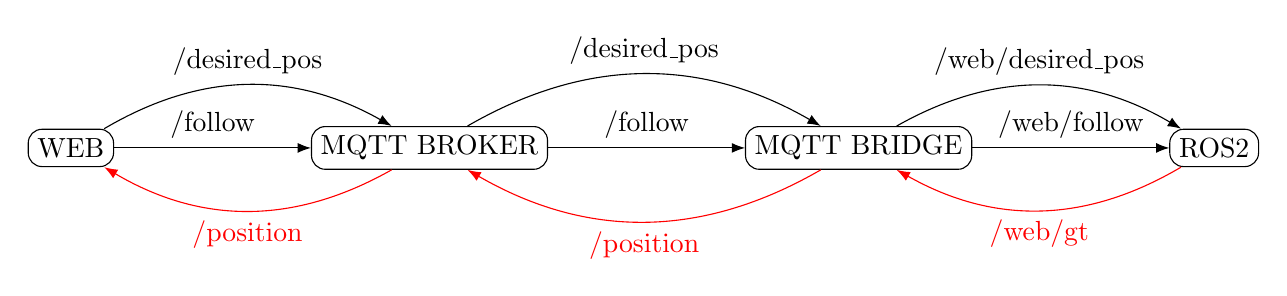
\begin{tikzpicture}[scale=1.4, node distance=2.5cm,>=Latex, mynode/.style={draw, rectangle, rounded corners=5pt}]
    % Definir nodos
    \node [mynode] (webserver) {WEB};
    \node [mynode, right=of webserver] (mqttbroker) {MQTT BROKER};
    \node [mynode, right=of mqttbroker] (mqttbridge) {MQTT BRIDGE};
    \node [mynode, right=of mqttbridge] (rosframework) {ROS2};
    
    % Dibujar líneas hacia adelante con nombre
    \draw[->] (webserver) -- (mqttbroker) node[midway, above] {/follow};
    \draw[->] (mqttbroker) -- (mqttbridge) node[midway, above] {/follow};
    \draw[->] (mqttbridge) -- (rosframework) node[midway, above] {/web/follow};
    \draw[->, bend left] (webserver) to node[midway, above] {/desired\_pos} (mqttbroker);
    \draw[->, bend left] (mqttbroker) to node[midway, above] {/desired\_pos} (mqttbridge);
    \draw[->, bend left] (mqttbridge) to node[midway, above] {/web/desired\_pos} (rosframework);
    
    % Dibujar línea hacia atrás con nombre
    \draw[->,red, bend left] (mqttbroker) to node[midway, below] {/position} (webserver);
    \draw[->,red, bend left] (mqttbridge) to node[midway, below] {/position} (mqttbroker);
    \draw[->,red, bend left] (rosframework) to node[midway, below] {/web/gt} (mqttbridge);
\hfill{}

\end{tikzpicture}
\end{center}
\caption{Esquema de flujo de datos desde la Web hasta ROS2}
\label{fig:esquema_flujo_datos}
\end{figure}


\section{Procesamiento de los mensajes MQTT a ROS2}
Por razones que se entenderán más avanzado el capitulo debemos procesar estos datos aún más, primero haciendo uso de un servicio de ROS2 
implementado por el paquete de robot\_localization, este transforma las coordenadas GPS expresadas en ángulos a un sistema cartesiano 
centrado en el punto de inicio y después debemos comprobar la distancia desde la posición actual del robot al punto que queremos ir, 
esto es debido a como funciona Nav2, si la distancia es menor a un valor dictado por los parámetros de Nav2 podemos enviarlo directamente 
al siguiente nodo, de no ser así generamos puntos equiespaciados desde la posición del robot hasta el objetivo y enviamos ese \textit{array} 
de posiciones, también cabe destacar que debemos generar una orientación deseada, cosa que la web no nos proporciona, para ello simplemente 
calculamos el ángulo que existe entre la posición del robot y la objetivo, para el caso de tener varios objetivos contiguos, es decir una 
ruta o camino hacemos este mismo algoritmo por cada par de puntos. El pseudo código se proporciona en el \textbf{algoritmo \ref{objetivos}}.

\begin{algorithm}[H]
  \caption{Procesamiento de objetivos}\label{objetivos}
  \begin{algorithmic}[1]
    \Procedure{Procesamiento}{JSONmsg} \Comment{calculo final de trayectoria genérica}
        \State $tipo\gets JSON.parse(JSONmsg)["type"]$
        \If{$tipo="marker" || tipo="follow"$}  
       
            \State $objetivo\gets JSON.parse(JSONmsg)["coordinates"]$
             \If{$dist(robot.position, objetivo) > rango $}
                \State $array\_objetivos \gets puntos\_intermedios(robot.position, objetivo, rango)$ 
                \State $publish(array\_objetivos)$
             \Else
                \State $publish(objetivo)$
             \EndIf
        \Else
            \For{$p \gets objetivos$} \Comment{hacemos lo mismo pero por cada 2 puntos del array}
                \If{$dist(p_0, p_1) > rango $}
                \State $array\_objetivos.push\_back( puntos\_intermedios(p_0, p_1, rango))$
             \Else
                \State $array\_objetivos.push\_back(objetivo)$
             \EndIf
            \EndFor
            \State $publish(array\_objetivos)$
        \EndIf
    \EndProcedure
  \end{algorithmic}
\end{algorithm}

Una vez procesada la información obtenida de la Web esta se publicará hacia otro nodo encargado de la lógica de control del paquete de 
navegación, este indicará a NAV2 donde ir y como, pero antes de ello debemos conseguir una localización estable en el tiempo.

\section{Localización y odometría}

La localización en robótica es uno de los problemas más explorados dada su importancia, por ello esta parte posiblemente sea la más 
importante del proyecto y la que mśa tiempo llevo conseguir.

Para ello se investigaron las mejores maneras de conseguir una buena localización en exteriores, donde a diferencia de los espacios cerrados 
esta tarea se vuelve un poco más compleja, existen métodos como SLAM o AMCL que funcionan muy bien en interiores pero cuando estas en un 
ambiente tan cambiante y con tan pocas referencias a las que puedas calcular tu posición estas alternativas se vuelven totalmente 
inútiles, principalmente tenemos 2 fuentes de odometría (IMU, Encoders de las ruedas) y 1 fuente de localización (GPS), existen múltiples 
opciones para conseguir una buena localización con estos dispositivos 
pero la que más usan los usuarios de ROS2 son sin duda los filtros de \textbf{Kalman} para fusionar múltiples fuentes de odometría 
 
EL \textbf{GNSS} (Global Navigation Satellite System) es una tecnología que funciona en base a hacer una triangulación con los satélites que 
estén a ''la vista'' en ese momento, normalmente esta 
posición es calculada por medio del estándar \textbf{WGS84}, eel cual es el último estándar creado para este propósito hasta la fecha, a 
diferencia de mucho de sus antecesores este tiene en consideración 
que la tierra no es perfectamente esférica sino elíptica. En la \textbf{figura \ref{fig:wgs84}} podemos ver el modelo WGS84 y sus sistema 
de referencia, este estaría en el cetro de la tierra 
con su eje \textbf{Z} apuntando al Norte y su eje \textbf{X} apuntando al primer meridiano.

\begin{figure}[h]
    \centering
    \includegraphics[width=0.5\textwidth]{images/wgs84.png}
    \caption{Sistema de referencia del modelo WGS84}
    \label{fig:wgs84}
\end{figure}

El principal problema de este sistema de referencia es que es bastante impráctico para la aplicación que aquí se discute, por ello 
necesitamos una transformación a sistema cartesiano y para ello debemos hablar también del sistema de coordenadas plano \textbf{UTM} 
(Universal Transverse Mercator), este es un sistema en base a la proyección de Mercator normal, pero en vez de hacerla tangente al Ecuador, 
se la hace secante a un meridiano y esta formado por 60 zonas que dividen el globo entero.  en la \textbf{figura \ref{fig:utm_europa}} se 
pueden observar tanto la nomenclatura de cada zona como su disposición.

\begin{figure}[h]
    \centering
    \includegraphics[width=0.5\textwidth]{images/europe_utm.png}
    \caption{Sistema de referencia del modelo UTM en Europa}
    \label{fig:utm_europa}
\end{figure}


A diferencia de las coordenadas geográficas este sistema se expresa en metros lo cual ya da una ventaja en cuanto a nuestra aplicación pero 
sigue habiendo el problema de que estas zonas son demasiado grandes por lo que también necesitamos calcular el \textit{offset} desde el 
origen de una de estas zonas a donde se inicie el robot, nos referiremos a este offset como \textit{Datum}.

Como podemos observar en la \textbf{figura \ref{fig:datum}} a parte de conocer la posición, necesitamos también el ángulo o \textit{bearing} 
y la declinación magnética, esta última es la que menos nos importa ya que es un dato que es bastante constante en el tiempo y varía por 
zona geográfica (varía alrededor de un 0,1\% al año), para el caso de málaga es de 0,061 rad.



\begin{figure}[h]
    \centering
    \includegraphics[width=0.5\textwidth]{images/navsat_transform.png}
    \caption{Sistema de referencia Datum}
    \label{fig:datum}
\end{figure}


Para ello tenemos también un paquete (robot\_localization) que nos 
ofrece una forma muy robusta de transformar los mensajes del GPS expresados en latitud y longitud (altitud la tomaremos igual a 0) a un 
sistema de referencia cartesiano, este nodo será \textbf{navsat\_transform} y básicamente se subscribirá a 3 topics para calcular 
el \textit{Datum} lo cual hará una sola vez y después en lo que se podría llamar el funcionamiento normal del nodo, publicara un mensaje 
\textit{nav\_msgs/Odometry} que será la transformación del GPS a coordenadas cartesianas. Para entender mejor el flujo de datos se incluye 
un esquema en la \textbf{figura \ref{fig:esquema_navsat}} y una explicación de las 3 suscripciones que necesita para trabajar.

\begin{itemize}
    \item un mensaje de \textit{sensor\_msgs/NavSatFix} con el mensaje proveniente del GPS, este será \textit{/hunter/fix}
    \item un mensaje de tipo \textit{nav\_msgs/Odometry} con la posición actual del robot y opcionalmente la orientación, está odometría 
será la salida de uno de los filtros de Kalman que utilizaremos para una mayor robustez en el sistema, esta información es necesaria por 
si el primer mensaje de GPS llega después de que el robot haya empezado a moverse, este será \textit{/odometry/global}.
    \item para este tercer mensaje lo que tenemos que proporcionar es la orientación global respecto al norte magnético y debe usarse la 
convención ENU (East, North, Up), que estipula un sistema de referencia con el este siendo el eje \textbf{x} y el norte el eje \textbf{y} 
como se puede observar en la \textbf{figura \ref{fig:wgs84}}, y para ello el nodo nos ofrece 4 maneras de hacerlo, la primera ya ha sido 
comentada y es usando la parte de orientación del primer mensaje de odometría y los otros 3 se listan a continuación.
        \begin{itemize}
            \item Una suscripción a un topic de tipo \textit{sensor\_msgs/Imu} con 9 grados de libertad, (ya que sin ellos no tenemos una 
orientación global respecto al norte magnético).
            \item Utilizar uno de los servicios que ofrece el paquete para que de manera externa calculemos ese datum y se lo enviemos, 
este servicio es \textit{/datum}.
            \item Indicarlo manualmente por medio de un archivo de parámetros en formato \textit{YAML}.
        \end{itemize}
\end{itemize}



\begin{figure}[h]
    

\begin{center}
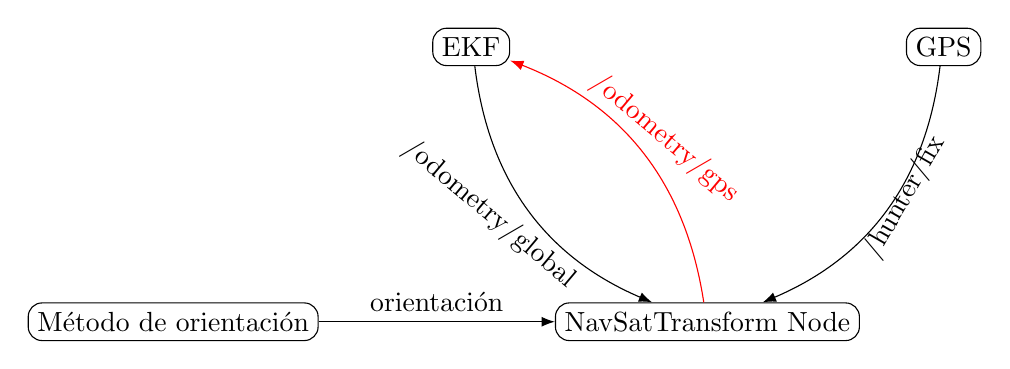
\begin{tikzpicture}[scale=1.4, node distance=3cm,>=Latex, mynode/.style={draw, rectangle, rounded corners=5pt}]

    \node [mynode] (navsat) {NavSatTransform Node};
    \node [mynode, above= of navsat, xshift = 3cm] (gps) {GPS};
    \node [mynode, above= of navsat, xshift = -3cm] (ekf) {EKF};
    \node [mynode, left=of navsat] (orient) {Método de orientación};
    \draw[->] (orient) -- (navsat) node[midway, above] {orientación};

    \draw[->, bend left] (gps) to node[pos=0.7, below right,rotate=60] {/hunter/fix} (navsat);
    \draw[->, bend right] (ekf) to node[pos=0.8, below left, rotate=-40] {/odometry/global} (navsat);
    
    \draw[->,red, bend right] (navsat) to node[pos=0.8, above right, rotate=-40] {/odometry/gps} (ekf);

\hfill{}

\end{tikzpicture}
\caption{Esquema de flujo de topics en el nodo navsat\_transform}
\label{fig:esquema_navsat}
\end{center}
\end{figure}

Al comienzo del proyecto como ya se ha comentado no se disponía de una IMU con orientación global por lo que se desarrollo un nodo que 
entre otras cosas calcula el ángulo respecto al norte magnético y lo transforma al sistema ENU antes de enviarlo por medio del servicio.
Para realizar este cálculo primero el nodo se suscribe al topic \textit{/hunter/fix} para las coordenadas GPS y al topic 
\textit{/hunter/odom} de tipo \textit{nav\_msgs/Odometry} para recibir información del movimiento del robot, también publicará por 
\textit{/cmd\_vel} para poder hacer mover al robot. 
Primero permanecemos a la espera de la llegada de un mensaje de GPS y guardamos estas coordenadas, posteriormente nos movemos una 
determinada distancia hacia delante, es decir solo en el eje \textbf{x} que será 
especificada por el usuario, y finalmente volveremos a esperar a otro mensaje del GPS. Por tanto para la posición tomaremos el segundo 
dato de GPS y para el cálculo de la orientación global,denotada como bearing o azimut seguiremos las siguientes ecuaciones.


\begin{equation}\label{eq:delta_longitud}
\Delta{l} =( \lambda_{2} - \lambda_{1} ) * (\pi/180) 
\end{equation}
\begin{equation}\label{eq:calculo_x}
X = cos(\phi_{2}) * sin(\Delta{l}), 
\end{equation}
\begin{equation}\label{eq:calculo_y}
Y = cos(\phi_{1}) * sin(\phi_{2}) - sin(\phi_{1}) * cos(\phi_{2}) * cos(\Delta{l})
\end{equation}
\begin{equation}\label{eq:calculo_bearing}
bearing = (\pi/2) - fmod((atan2(Y,X) + 2\pi),2\pi)
\end{equation}

Las siguientes ecuaciones describen el cálculo del rumbo (bearing) entre dos puntos geográficos, dados por sus coordenadas de 
latitud (\(\phi_1, \phi_2\)) y longitud (\(\lambda_1, \lambda_2\)):

Donde:
\begin{itemize}
    \item \(\Delta{l}\) es el cambio en longitud, medida en radianes.
    \item \(X\) es una componente del cálculo intermedio.
    \item \(Y\) es otra componente del cálculo intermedio.
    \item \({bearing}\) es el rumbo entre los dos puntos, medido en radianes.
    \item \(\pi\) es la constante pi, aproximadamente 3.14159.

\end{itemize}

Fijándonos en la \textbf{ecuación \ref{eq:calculo_bearing}}, podemos observar que hacemos el modulo del angulo con 360º, esto es debido 
a que la función atan2 devuelve un valor en el rango $[ \pi/2,\pi/2 ]$, y nosotros lo queremos en
el rango $[0, 2\pi]$, también como hemos comentado el ángulo debe estar acorde al sistema ENU y por tanto le restamos $\pi/2$. Finalmente 
lo enviamos al servicio y el nodo a partir de aquí comienza a funcionar.

Por último falta la configuración de los EKF, para esta implementación tomaremos también el mismo paquete que no ofrece la posibilidad de 
configurarlos de una manera sencilla.

El principal problema que se considera aquí es la diferencia entre la localización y la localización, donde la primera es muy rápida, 
(más de 30 Hz) y precisa para intervalos de tiempo muy cortos, es decir \textit{deriva} mucho con el tiempo y por otro
lado la localización proporcionada por el GPS que es muy lenta, discreta, da saltos discretos en el tiempo y por tanto no vale para usar en 
intervalos cortos de tiempo pero es extremadamente precisa en intervalos muy largos, está es una fuente por definición no tiene
\textit{deriva} en el tiempo, por tanto necesitamos de las dos para conseguir una buena localización.

Para ello empezaremos creando una instancia de un filtro de Kalman para las fuentes continuas (Odometrías), este lo llamaremos 
\textit{ekf\_local} ya que lo usaremos para navegación y planificación de movimientos en el sistema de referencia \textit{/odom}, estos 
filtros funcionan con matrices de 15 variables para cada fuente de odometría  , estás son: 
$[ X,Y,Z,\theta_{x},\theta_{y},\theta_{z},\dot{X},\dot{Y},\dot{Z},\dot{\theta_{x}},\dot{\theta_{y}},\dot{\theta_{z}},\ddot{X},\ddot{Y},\ddot{Z} ]$,
pero ya que tomaremos que estamos trabajando en 2 dimensiones (por ser un robot terrestre y Ackermann hay mucho movimientos que podemos 
ignorar), de esta manera las variables que tenemos que tener en cuenta serian: 
$[ X,Y,\theta_{z},\dot{X},\dot{Y},\dot{\theta_{z}},\ddot{X},\ddot{Y}]$. Pero se puede ir más, allá primero con el pensamiento lógico en 
cuanto al hardware, no todos los dispositivos nos proporcionan todas estas variables y eso está bien no lo necesitamos, sino que para que 
el filtro funcione correctamente y no empiece a oscilar descontroladamente (comúnmente llamado ''explotar''), necesitamos que que entre 
todas las fuentes
tengamos las variables necesarias, estás variarán mucho según cada situación, como los sensores de los que se dispongan, su precisión, el 
tipo del robot o incluso el entorno en el que el robot se mueva, esta tarea puede volverse sorprendentemente compleja
y por ello se han desarrollado una seria de ''normas'' que nos indican que variables introducir y como. Estás normas son fruto de múltiples 
fuentes de información como la documentación oficial del paquete usado y la charla sobre el mismo dada por su creador en la ROSCon 
(ROS conference) del 2015, exhaustiva investigación por internet de múltiples usuarios y por último muchas horas de pruebas en el terreno 
con el propio robot. Otro dato importante a resaltar es que estas 5 normas tiene una prioridad, esto quiere decir que si alguna se 
contradice siempre debemos priorizar a la siguiente.  

\begin{enumerate}
    \item Siempre que podamos debemos introducir variables directamente medidas, esto significa que si por ejemplo tenemos un sensor que 
mide la velocidad de las ruedas y en base a eso calcula su posición, una mejor práctica es introducir la velocidad.
    \item Para que el filtro sea estable, mínimo necesitamos introducir una \textit{pose} completa, que para nuestro caso de robot Ackermann 
sería, $[ X,Y,\theta_{z}]$, si eso no es posible entonces debemos proporcionar sus respectivas velocidades.
    \item Si tenemos una fuente de velocidad lineal y posición, una mejor práctica es proporcionar la velocidad lineal y por otro lado si 
esa fuente proporciona velocidad angular y orientación la mejor práctica es introducir la orientación.
    \item Las matrices de covarianza que incluyen los mensajes que proporcionamos al filtro son extremadamente importantes ya que indican 
cuando usar una variable o cuando usar otra, nunca debemos introducir una variable donde su varianza no haya sido calculada o esta sea 0, 
tampoco debemos introducir 2 fuentes de la misma variable (solo para el caso de orientación y posición) que tengan el mismo o muy parecido 
valor de varianza, ya que esto causará un rápido cambio entre los dos valores que puede llegar a una oscilación indeseada en la salida del 
filtro.
    \item Debemos analizar las restricciones de nuestro tipo de robot en particular, (Ackermann, diferencial, omnidireccional, etc...). 
Para nuestro caso, Ackermann, sabemos que este no puede tener un cambio instantáneo en el eje \textbf{y} y por tanto $\dot{Y}$ siempre va 
a ser 0, podríamos pensar que no debemos introducir esta variable pero esto no es así ya que introduciendo este valor le estamos 
''indicando'' al filtro que este no se puede mover en esa dirección, también podríamos pensar lo mismo para $\ddot{Y}$, pero dado que los 
valores de esta variable suelen venir de una IMU y sabiendo que estas normalmente proporcionan una cantidad de ruido demasiado grande la 
mejor práctica en este caso en no proporcionarla.
\end{enumerate}

Dadas estas normas se llegó a la siguiente configuración. Para la odometría de las ruedas se introdujo 
$[ \dot{X},\dot{Y},\dot{\theta_{z}} ]$ y para la IMU $[ \theta_{z},\dot{\theta_{z}},\ddot{X},\ddot{Z} ]$. De está manera no solo cumplimos 
con todos los criterios mencionados sino que tenemos duplicidad en múltiples variables lo que hace al filtro mucho más robusto. Este filtro 
a parte de tener como salida una publicador de un mensaje tipo \textit{nav\_msgs/Odometry} con las entradas fusionadas también nos 
proporciona la transformación de \textit{/odom} a \textit{/base\_link} dejándonos así un paso más cerca de conseguir todo el árbol de 
transformaciones como se puede visualizar en la \textbf{figura \ref{fig:arbol_urdf}}.

Posteriormente se introdujo el segundo filtro de Kalman al que 

Una vez comprobado en el terreno que el filtro funcionaba, se introduce una segunda instancia del filtro de Kalman, esta será nombrada como 
\textit{ekf\_global} y su salida solo será usada para realimentar al nodo de \textbf{NavSatTransform} como se ve en la 
\textbf{figura \ref{fig:esquema_localizacion}}


\begin{figure}[h]
    

\begin{center}
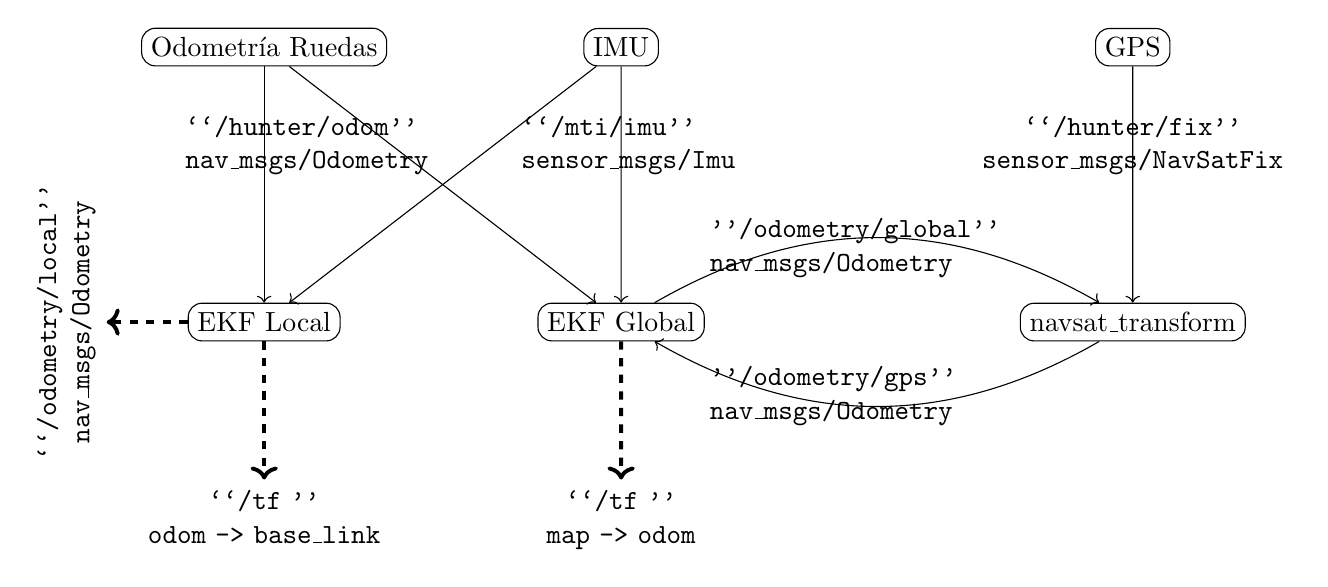
\begin{tikzpicture}[scale=0.2,node distance=0.5cm and 1cm,mynode/.style={draw, rectangle, rounded corners=5pt}]
    \node [mynode] (ekf_local) {EKF Local};
    \node [mynode, right = 2.5cm of ekf_local] (ekf_global) {EKF Global};
    \node [mynode, right = 4cm of ekf_global] (navsat) {navsat\_transform};
    \node [mynode, above = 3cm of ekf_local] (odometria_hunter) {Odometría Ruedas};
    \node [mynode, above = 3cm of ekf_global] (imu) {IMU};
    \node [mynode, above = 3cm of navsat] (gps) {GPS};
    \draw[->] (odometria_hunter) -- (ekf_local) node[midway, above, text width=2cm, align=center] {\texttt{``/hunter/odom'' nav\_msgs/Odometry}};    
    \draw[->] (odometria_hunter) -- (ekf_global) node[] {};    
    \draw[->] (gps) -- (navsat) node[midway, above, text width=4cm, align=center] {\texttt{``/hunter/fix'' sensor\_msgs/NavSatFix}};    


    \draw[->] (imu) -- (ekf_local) node[midway, above, text width=-2cm, align=center] {\texttt{``/mti/imu'' sensor\_msgs/Imu}};    
    \draw[->] (imu) -- (ekf_global) node[] {}; 

    \draw[->, bend left] (ekf_global) to node[pos=0.3,text width=2cm, align=center] {\texttt{''/odometry/global''  nav\_msgs/Odometry}} (navsat);

    \draw[->, bend left] (navsat) to node[pos=0.7,text width=2cm, align=center] {\texttt{''/odometry/gps''  nav\_msgs/Odometry}} (ekf_global);


    \draw[->, dashed,line width=0.5mm] (ekf_local) -- +(-10, 0) node[above,rotate=90,text width=4cm, align=center] {\texttt{``/odometry/local'' nav\_msgs/Odometry}};

    \draw[->, dashed,line width=0.5mm] (ekf_local) -- +(0, -10) node[below,text width=4cm, align=center] {\texttt{``/tf  '' \\ odom -> base\_link}};
    \draw[->, dashed,line width=0.5mm] (ekf_global) -- +(0, -10) node[below,text width=4cm, align=center] {\texttt{``/tf  '' \\ map -> odom}};

    
\end{tikzpicture}
\caption{Esquema de topics completo sobre el funcionamiento de la localización}
\label{fig:esquema_localizacion}
\end{center}
\end{figure}

Para el caso de las entradas de fuentes de odometría de este filtro serán las mismas con la misma configuración que para el 
\textit{ekf\_local}, pero con la diferencia de que ahora añadiremos la salida del nodo \textit{navsat\_transform}, está es 
\textit{/odometry/gps} como se explica en la \textbf{figura \ref{fig:esquema_localizacion}}, para está añadiremos si o si las 
componentes X e Y ya que son las únicas que tiene este topic y a parte son las únicas que nos interesan,
 estás nos darán una localización que se mantenga en el tiempo pero con saltos discretos.

Con estos tendríamos solucionado el problema de la localización y así se podría pasar a la realización e implementación del ''stack'' 
de navegación.

\section{Navegación Autónoma haciendo uso de Nav2}
 \cleardoublepage


\chapter{Pruebas y resultados}

\chapter{Conclusiones}

\chapter{Futuras líneas de trabajo}